\documentclass{article}

\usepackage{graphicx}
\usepackage{tikz}
\usepackage{tikzsymbols}
\usetikzlibrary{calc,patterns,shapes.geometric}
\pagestyle{empty}
\usepackage[margin=0pt]{geometry}
\geometry{papersize={14in,12in}}

\def\centerarc[#1](#2)(#3:#4:#5){\draw[#1] ($(#2)+({#5*cos(#3)},{#5*sin(#3)})$) arc (#3:#4:#5);}

\begin{document}
	\begin{figure}
		\centering
		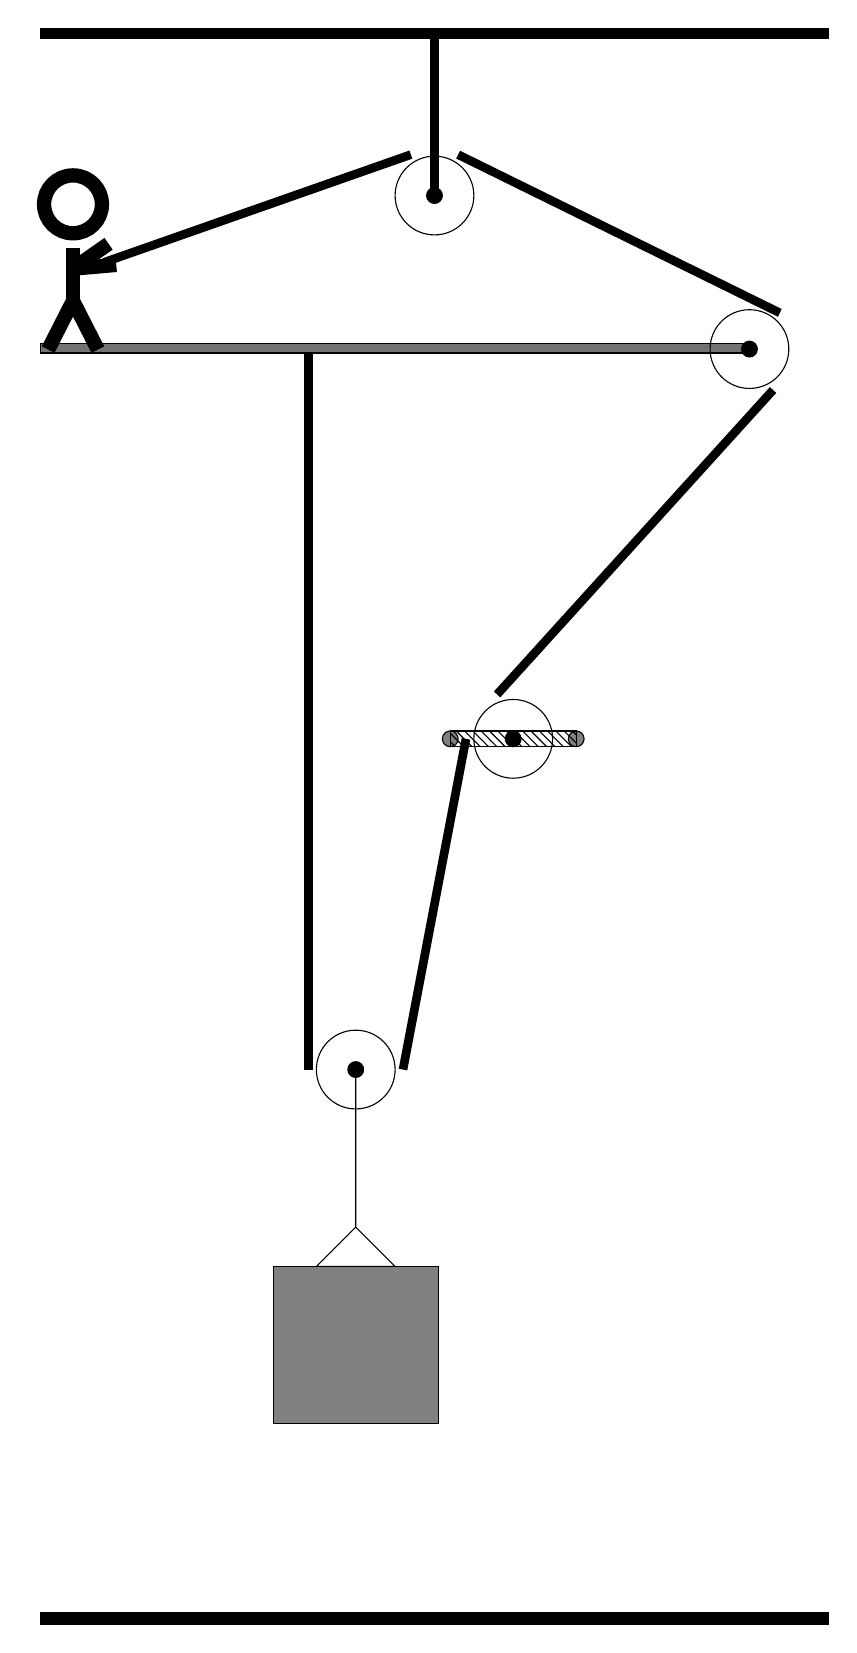
\begin{tikzpicture}
			%%%%% START %%%%%
			\draw[fill=black] (-2, 18) rectangle (8, 18.125);
			
			\draw[fill=black!55] (-2, 14) rectangle (7, 14.125);
			
			\draw (2, 4.9) circle (0.5);
			\draw[fill=black] (2, 4.9) circle (0.1);
			
			\draw (7, 14.05) circle (0.5);
			\draw[fill=black] (7, 14.05) circle (0.1);
			
			\draw[fill=white](4, 9.1) circle (0.5);
			\draw[fill=black] (4, 9.1) circle (0.1);
			\draw[fill=black!50] (3.2, 9.1) circle (0.1);
			\draw[fill=black!50] (4.8, 9.1) circle (0.1);
			\draw[pattern=north west lines, pattern color=black] (3.2, 9.2) rectangle (4.8, 9.0);
			
			\draw (3, 16) circle (0.5);
			\draw[fill=black] (3, 16) circle (0.1);
			\draw[line width=1.1mm] (3, 16) -- (3, 18);
			
			\draw (2, 4.9) -- (2, 2.9) -- (1.5, 2.4) -- (2.5, 2.4) -- (2, 2.9);
			\draw[fill=black!50] (0.95, 2.4) rectangle (3.05, 0.4);
			
			\draw[line width=1.1mm] (1.4, 14) -- (1.4, 4.9);
			\centerarc[line width=1.1mm](2, 4.9)(180:360:0.6);
			\draw[line width=1.1mm](2.6, 4.9) -- (3.4, 9.1);
			\centerarc[line width=1.1mm](4, 9.1)(110:180:0.6);
			\draw[line width=1.1mm](3.7948, 9.6638) -- (7.3, 13.5304);
			\centerarc[line width=1.1mm](7, 14.05)(-60:50:0.6);
			\draw[line width=1.1mm](7.3857, 14.5096) -- (3.3, 16.5196);
			\centerarc[line width=1.1mm](3, 16)(60:120:0.6);
			\draw[line width=1.1mm](2.7, 16.5196) -- (-1.2, 15.15);
			
			\node at (-1.5, 15.15) {\Strichmaxerl[10][-175][35]};
			
			\draw[fill=black] (-2, -2) rectangle (8, -2.15);
			%%%%% END %%%%%
		\end{tikzpicture}
	\end{figure}	
\end{document}